\chapter{Objetivos y Metodología de Trabajo}

Este capítulo detallará los objetivos impuestos tras el trabajo de análisis inicial que se pretende alcanzar mediante los periodos de investigación e implementación de esta tésis de fin de Máster. Se describirá brevemente lo que se quiere abordar y cómo se pretende hacer, además de incluir otros sub-objetivos que surgieron durante el desarrollo reservando los detalles de los mismos para el punto en el que sea relevante. Así mismo, se expondrá la metodología bajo la que se organizó el proyecto.

\section{Proyecto Planteado}

Esta sección se reserva para exponer la idea objeto de esta tesis y la motivación o motivaciones principales que han llevado a su desarrollo, de vital importancia para comprender qué se pretende conseguir con ella y por qué se escogió esta idea y no otra.

La \textbf{``Ejecución Mixta''} para proyectos de robótica y visión artificial surge de la conjunción de las ideas planteadas en el capítulo anterior, persiguiendo incrementar la accesibilidad de la robótica y su aprendizaje. Se busca elaborar una herramienta que pueda ser conectada de manera modular con cualquier aplicación de carácter robótico y con soporte para cualquier usuario, sean cuales sean sus circunstancias.

Esta idea se planteó como una serie de características intrínsecas que dan forma a los objetivos que se quiere lograr. En tanto que se quiere facilitar el uso de la robótica, deberá existir un Interfaz de Programación o API que abstraiga a los usuarios de todo lo relacionado con la infraestructura de la herramienta y la aplicación, de los mecanismos de comunicación con los sistemas involucrados (tanto robots como sensores y PCs, servidores, \textit{proxys}, etc.) y del control de flujo propio de un sistema complejo, permitiéndole centrarse en su tarea específica de desarrollar con robots. Además, dado que los usuarios potenciales no desean suponer costes sobre los constructores de las aplicaciones que necesitan usar para su trabajo o estudio y que tampoco quieren que se les cobre su utilización (debido en muchos casos a que no se pueden afrontar tasas a largo plazo sin resultados prometedores en plazo corto), la idea que se expone debe estar orientada al cliente, siendo este el que acarree con toda la carga de cómputo posible y asuma el consumo de recursos, que utilizará a su conveniencia según la disponibilidad de la que goce.

La herramienta final objetivo constituirá una forma de lograr no sólo la ejecución de código específico accediendo a un único elemento \textit{hardware} concreto de la máquina cliente, sino la ejecución de aplicaciones robóticas completas de cualquier ámbito en cualquier dispositivo \textit{hardware} del que el cliente disponga, incluso si éste está conectado a través de un puerto USB o una red WiFi (ya sea un ordenador, sensores, un robot, etc.) mientras el código se almacena remotamente y se ofrece al usuario a través de la nube, por medio de las tecnologías web. Bajo esta filosofía el código o la aplicación desarrollada por el cliente a través de la web se almacena en un servidor remoto, pero éste sigue teniendo acceso a su análisis y resultados al ejecutarse en sus propios equipos y sistemas robóticos locales, quedando todas las tareas de bajo nivel involucradas en la aplicación robótica ``escondidas'' a nivel de usuario y solventadas por la aplicación que se sirve, como puede ser la comunicación entre servidor y cliente y el acceso a su \textit{hardware}, el diálogo entre el código implementado y robot (simulado o real) y con lo relacionado con el soporte gráfico (UI) y el entorno de trabajo, de modo que se dota al usuario de cierta abstracción de los temas que para él o ella son irrelevantes, permitiéndole centrar sus esfuerzos en idear y desarrollar la lógica que controle al robot y le permita abordar el problema que se propone.

La herramienta deberá encajar con aplicaciones docentes y de investigación, actuando más bien como una capa intermedia que hace las funciones de \textit{middleware} entre el robot del usuario y un sistema remoto.

\section{Objetivos del Proyecto}

Este trabajo esta compuesto por cuatro grandes objetivos impuestos en primera instancia, pudiendo todos ellos descomponerse a su vez en sub-objetivos de menor complejidad que sirven para disponer un escenario de trabajo inicial:

\begin{enumerate}
\item Realizar un profundo trabajo de investigación acerca de las herramientas, componentes y entornos más utilizados en los proyectos robóticos.
    \begin{itemize}
        \item Se trata de analizar las características de cada agente de estudio para poder elegir o descartar con criterio su incorporación al proyecto.
    \end{itemize}
\item Probar y seleccionar aquellas herramientas que puedan adaptarse al problema que se pretende resolver.
    \begin{itemize}
        \item Este hito pasa por construir diseños preliminares del entorno que engloba un cliente y un sistema remoto que se quieren interconectar.
    \end{itemize}
\item Construir una nueva solución en forma de módulo que resuelva un problema para el que aún no existe una solución clara.
    \begin{itemize}
        \item Este proceso supone a su vez la implementación de prototipos,
        \item nuevas etapas de investigación para el enriquecimiento del sistema y
        \item continuos procesos de supervisión para asegurar que el resultado contiene las características objetivo, que son:
            \begin{itemize}
                \item Accesible (Multiplataforma, Multilenguaje).
                \item Soporte para simulación y sistemas reales.
                \item Ejecución en el cliente.
                \item Fácil de usar.
                \item Versátil (Visión Artificial, Robots de cualquier clase).
            \end{itemize}
    \end{itemize}
\item  Llevar a cabo un exhaustivo programa de pruebas para evaluar la validez y la viabilidad de la idea planteada y su implementación.
\end{enumerate}

Estos objetivos establecen a su vez un esquema de trabajo que dictará la manera en que se desarrolla, realizando siempre una supervisión para garantizar que se cumple cada meta propuesta antes de pasar a la siguiente.

\section{Metodología Empleada}

Este proyecto se dividirá, principalmente, en dos partes bien diferenciadas: \textbf{etapa de investigación} y \textbf{etapa de implementación}. Estableceremos de antemano una serie de reglas que organizarán la manera en que se trabaja en ambas partes en busca de la mayor eficiencia y efectividad posible.

En cuanto al método de sincronización del trabajo se puede decir que se descompuso su elaboración en una serie de iteraciones fromadas por varias fases en las que, por medio de una reunión, se pusieron en común los avances obtenidos en cada período para evaluar el estado del proyecto y corregir posibles fallos, además de establecer los sub-objetivos siguientes, discutir la mejor manera de abordarlos y determinar los obstáculos que podían surgir de cara a la siguiente iteración. Esto no sólo constituye un método de trabajo fluido y completo, sino que además permite asentar bien los conocimientos adquiridos y puestos en práctica para resolver cada problema. Gracias a esta rápida realimentación, los errores no se propagan y las dudas se despejan con gran eficacia. Durante los intervalos de trabajo entre cada reunión, el seguimiento se hizo a través de una bitácora semanal \footnote{\url{https://github.com/cawadall/TFM-Carlos-Awadallah/blob/master/README.md}} donde se iba actualizando asiduamente el estado del proyecto a través de material audiovisual, \textit{snippets} de código y detalladas descripciones de lo hecho. Tanto esta bitácora como el código del proyecto, de carácter abierto, estuvo en todo momento accesible para los tutores, con lo cual se podían preparar las reuniones de antemano e incluso intercambiar ideas y sugerencias de manera anticipada \footnote{\url{https://github.com/cawadall/TFM-Carlos-Awadallah}}.

\subsection{Metodología de Investigación}

Dado que estamos tratando de abordar un problema para el que aún no existe una solución, gran parte del proyecto se dedicó a la investigación. Se hizo necesario reunir la documentación asociada a una gran cantidad de herramientas y proyectos en auge que reunían algunas de las características que buscábamos. Para abordar esta parte del trabajo, tratamos de realizar una primera pasada escogiendo todas aquellas opciones que contaran con al menos una de las características que habíamos establecido como objetivo. A partir de este punto, realizamos numerosos ciclos, cada uno de ellos con su respectivo proceso de testeo, para filtrar en primera instancia todas aquellas que fueran poco maduras, incompletas o que no encajasen con los requisitos de nuestro proyecto, y luego se trató de descartar, en un último ciclo, los peores candidatos entre las herramientas finalistas en base a una evaluación del porcentaje de superposición entre el conjunto de prestaciones de la herramienta y el set de características que habíamos establecido.

Esta filosofía se respetó hasta el comienzo de la implementación punto a partir del cual cualquier tarea que requiriese volver a investigar se produjo simplemente con la idea de resolver un problema muy concreto o mejorar algún punto del trabajo.

\subsection{Metodología de Implementación}

Para la consecución del resto de objetivos se optó por la filosofía de Barry Boehm del modelo de desarrollo en espiral \cite{BB1986}. Este método busca separar el comportamiento objetivo en diferentes sub-tareas de menor complejidad conservando la flexibilidad ante nuevos objetivos que surjan durante el desarrollo o sucesos no previstos y requisitos variantes, circunstancias que suelen estar presentes en la mayoría de proyectos de este calibre. Así, se consigue fijar la arquitectura y el flujo de trabajo en la fase inicial e ir construyendo la aplicación gradualmente mientras se verifica simultáneamente la calidad en cada paso (Fig. \ref{espiral_bb}).

\begin{figure}[!htbp]  \centering\noindent
    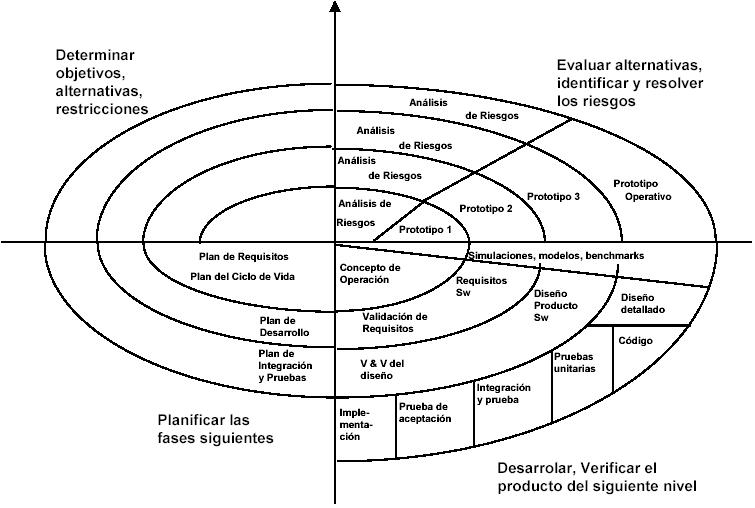
\includegraphics[width=0.95\textwidth]{figures/espiral_boehm.jpg}
    \caption{Modelo en Espiral del Proceso de Desarrollo Software.}
    \label{espiral_bb}
\end{figure}

Gracias a la estructura cíclica se consigue tener un prototipo funcional que va creciendo en riqueza y complejidad en cada pasada, construyéndose cada vez sobre el prototipo de la iteración anterior para abordar los objetivos de ciclo, a través de los cuales se consigue mejorar el desarrollo y, en última instancia, pulirlo para cubrir todos los requisitos planteados y obtener la versión final. Cada fase del desarrollo incremental se divide en 4 fases bien definidas por las que el proyecto debe pasar:
\begin{enumerate}
    \item \textbf{Determinar los objetivos del ciclo}. Esta primera fase consiste en definir las metas que se pretende alcanzar en el ciclo. Estas metas son a su vez las que determinan cuándo se da por finalizada la iteración.
    \item \textbf{Análisis del riesgo}. En segundo lugar se trata de analizar los objetivos propuestos en búsqueda de las partes más delicadas para determinar qué problemas u obstáculos pueden surgir durante el desarrollo y planificar cómo abordarlos.
    \item \textbf{Desarrollar y probar}. Con un plan de desarrollo definido en base a los riesgos potenciales, y con los objetivos de ciclo presentes, se comienza con la implementación. También ha de pasarse el correspondiente \textit{set} de pruebas para garantizar un desarrollo funcional y completamente operativo.
    \item \textbf{Planificación de la siguiente fase}. Para acabar, se evalúan los resultados obtenidos en la etapa actual del proyecto y se comienza con la planificación de las próximas fases del proyecto.
\end{enumerate}
